\documentclass[12pt, twoside]{article}
\usepackage[francais]{babel}
\usepackage[T1]{fontenc}
\usepackage[latin1]{inputenc}
\usepackage[left=7mm, right=7mm, top=4mm, bottom=4mm]{geometry}
\usepackage{float}
\usepackage{graphicx}
\usepackage{array}
\usepackage{multirow}
\usepackage{amsmath,amssymb,mathrsfs} 
\usepackage{soul}
\usepackage{textcomp}
\usepackage{eurosym}
\usepackage{lscape}
 \usepackage{variations}
\usepackage{tabvar}
 
\pagestyle{empty}




\begin{document}

\begin{center}
 \textbf{\Large{\ul{Proportionnalit�}}}
\end{center}

\enskip

\textbf{\large{1. D�finitions}}

\enskip

\ul{D�finition}: Dire que deux grandeurs sont proportionnelles revient � dire
que les valeurs de l'une s'obtiennent en multipliant les valeurs de l'autre
par un m�me nombre appel� \textbf{coefficient de proportionnalit�}.

\enskip


\ul{D�finition}: Un \textbf{tableau de proportionnalit�} est un tableau
repr�sentant deux grandeurs proportionnelles.

\enskip

\ul{Exemple}: 

\enskip


\begin{tabular}{|c|c|c|c|c|c|}
\hline
c�t� du carr� en cm & \quad 1 \quad & \quad 2 \quad & \quad 3 \quad & \quad 6
\quad & \quad 10 \quad \\
\hline
p�rim�tre en cm & \quad & \quad & \quad & \quad &\quad \\
\hline
\end{tabular}

\bigskip

\textbf{\large{2. Calculer une quatri�me proportionnelle}}


\enskip

\ul{Exemple}: Le prix du pain est proportionnel au nombre de baguettes achet�es.

\bigskip


\textbf{M�thode 1: En utilisant le coefficient de proportionnalit�}

\enskip


\begin{tabular}{|c|c|c|c|}
\hline
nombre de baguettes & \quad 1 \quad & \quad 3 \quad  & \quad 4 \quad \\
\hline
prix en \euro & \quad 0,87 \quad & \quad 2,61 \quad  & \quad \ldots \ldots \quad \\
\hline 
\end{tabular}


\bigskip

\textbf{M�thode 2: En utilisant les op�rations dans un tableau de
proportionnalit�}

\enskip

\ul{Propri�t�}: Dans un tableau de proportionnalit�, on peut construire une
nouvelle colonne:

\begin{itemize}
  \item [$\bullet$] en \textbf{multipliant} les valeurs d'une colonne par un
  m�me nombre;
  \item [$\bullet$] en \textbf{divisant} les valeurs d'une colonne par un
  m�me nombre; 
  \item [$\bullet$] en \textbf{ajoutant} les valeurs de deux colonnes ensemble. 
\end{itemize}

\bigskip



\begin{tabular}{cc}
\begin{minipage}{8cm}
\begin{tabular}{|c|c|c|}
\hline
nombre de baguettes  & \quad 4 \quad & \quad 8 \quad   \\
\hline
prix en \euro & \quad 3,48 \quad   & \quad \ldots \ldots \quad \\
\hline 
\end{tabular}


\end{minipage}
&
\begin{minipage}{10cm}
\begin{tabular}{|c|c|c|c|}
\hline
nombre de baguettes  & \quad 3 \quad & \quad 5 \quad  & \quad 8 \quad \\
\hline
prix en \euro & \quad 2,61 \quad & \quad 4,35 \quad  & \quad \ldots \ldots \quad
\\
\hline 
\end{tabular}
\end{minipage}
\end{tabular}

\bigskip

\textbf{M�thode 3: En utilisant la r�gle ``d'�galit� des produits en
croix''}

\enskip

\begin{tabular}{|c|c|c|}
\hline
nombre de baguettes  & \quad 3 \quad  & \quad 7 \quad \\
\hline
prix en \euro & \quad 2,61 \quad  & \quad x \quad \\
\hline 
\end{tabular}

\bigskip

\textbf{\large{3. Repr�sentation graphique}}

\enskip

\fbox{\begin{minipage}{18cm}
Une situation de proportionnalit� est repr�sent� graphiquement par des
\textbf{points align�s} sur une droite \textbf{passant par l'origine des axes}.
      \end{minipage}
}


\enskip

\ul{Exemple}:


\begin{center}
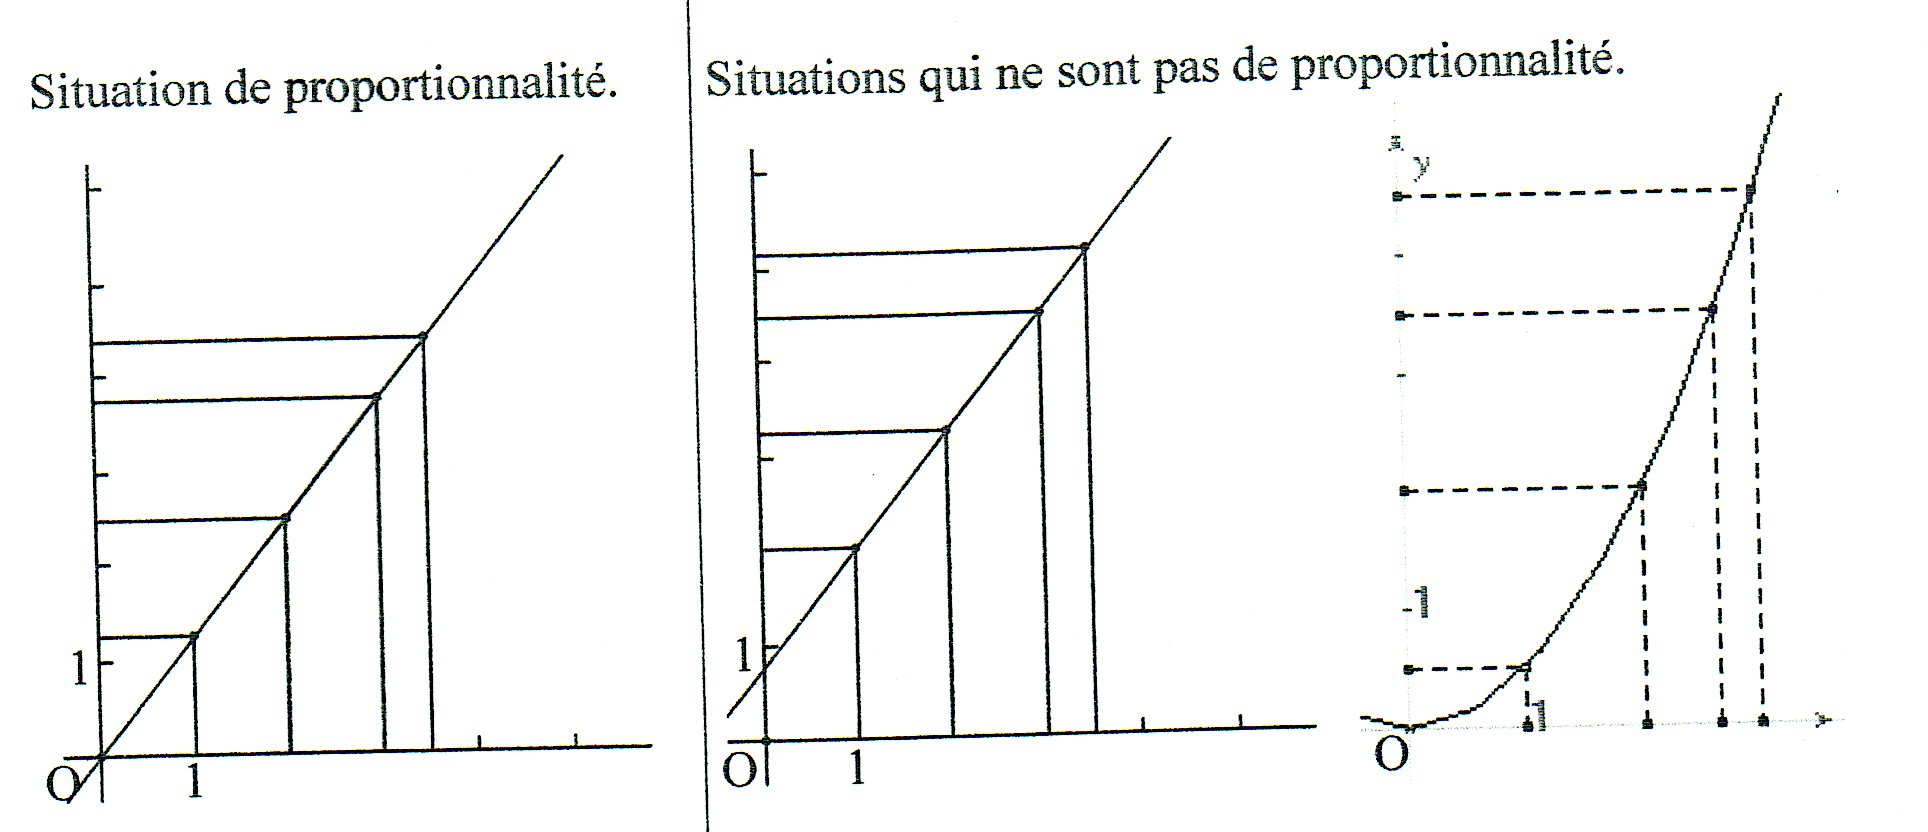
\includegraphics[width=12cm]{images/graphes.jpg}
\end{center}


\end{document}
